\subtop{Techniken für Textdaten}{-1.725}
\begin{description}
	\item[Schwierigkeiten] \ \\\vspace*{-\baselineskip}
		\begin{itemize}
			\item nicht pre-attentive
			\item abstrakt
			\item sehr hoch-dimensional
			\item Aufbau (sehr unterschiedlich möglich)
			\item subtil
		\end{itemize}
	\item[Stationen] \ \\\vspace*{-0.5\baselineskip}\\
	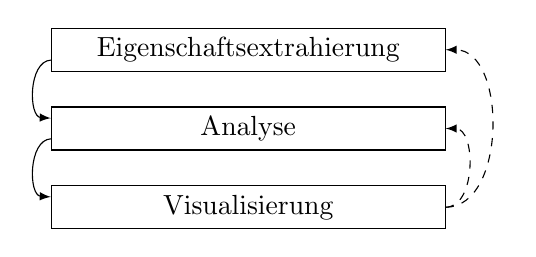
\begin{tikzpicture}[every node/.style={draw, minimum width=5cm}]

\node (e) at (0,0) {Eigenschaftsextrahierung};
\node (a) at (0,-1) {Analyse};
\node (v) at (0,-2) {Visualisierung};

\draw[->, >=latex] (e) to[out=183, in=177] (a);
\draw[->, >=latex] (a) to[out=183, in=177] (v);
\draw[->, >=latex, dashed] (v) to[out=0, in=0] (e);
\draw[->, >=latex, dashed] (v) to[out=0, in=0] (a);
\end{tikzpicture}
	\item[Beispiele] \ \\\vspace*{-\baselineskip}
		\begin{description}
			\item[InkBlots] Texteigenschaft-Visualisierung \\
				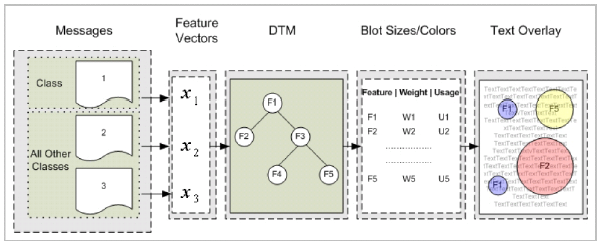
\includegraphics[width=0.9\textwidth]{Pics/03-02-InkBlots.png}
		\end{description}
\end{description}
\topbreak
\begin{description}
	\item \ \\\vspace*{-\baselineskip}
		\begin{description}
			\item[Plagiaterkennung] Strukturanalyse
			\item[Cloudlines Text and Geo] visuelle Event Analyse\\
			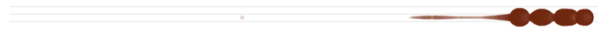
\includegraphics[width=0.9\textwidth]{Pics/03-02-Cloudlines.png}
		\end{description}
\end{description}